%!TEX root = main.tex
\section{Introduction}
%This chapter explains the motivation behind the project and the importance to test and benchmark the different available platforms from cloud providers. It introduces the topics of cloud computing and particularly serverless computing and briefly explains the term benchmarking.
%\subsection{Motivation}
%In today's world cloud computing is for many companies and organizations a good and maybe the best option to set up their computing infrastructure or migrate to it. 
%Smaller or newer companies often cannot afford to invest in high-performance hardware which they also need to manage themselves. Sometimes companies don't have the knowledge to maintain hardware properly and just want their databases and web servers to work, instead of worrying about a hardware failure or a power outage. 
%Furthermore most businesses want to focus on their core business which many times means using computing resources and tools instead of managing them.\\
%This thesis is going to investigate a specific region of cloud computing; generally known as 
The serverless computing paradigm is an emerging approach to develop cloud-based applications~\cite{Baldini2017, riseofserverless, vanEyk:2017:SCG:3154847.3154848}.
\gls{IBM}~\cite{serverlessibm} defines it as \emph{"an approach to computing that offloads responsibility for common infrastructure management tasks (scaling, scheduling, patching, provisioning, etc.) to cloud providers and tools, allowing engineers to focus their time and effort on the business logic specific to their applications or process"}.\vs{nicer way to report quote?}
Serverless requires less expertise than other self-managed approaches.
Users don't manage directly the infrastructure and runtime of the system, delegating its operations to the cloud provider.
Additionally, cloud providers can deploy finer-grain billing policies (\emph{e.g.}, on a per service-call basis) for any of the offered services~\cite{serverlessaws, serverlessazure}, generally leading to reduced costs for developers.

\begin{figure}[!t]
\begin{center}
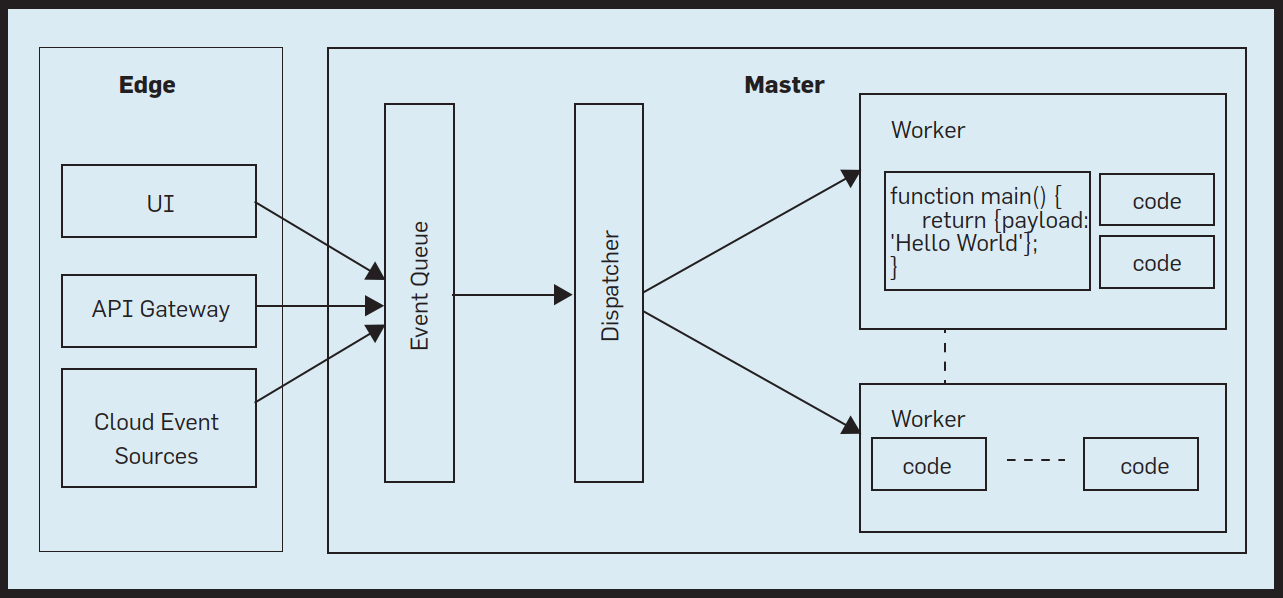
\includegraphics[scale=0.2]{bilder/FaaS_architecture.png}
\captionsetup[table]{justification=centering, labelfont=bf}
\caption{\vs{TO REDO: identify which components are being benchmarked} Typical FaaS architecture.\label{fig:faas_arch}}
\end{center}
\end{figure}
%Using serverless technologies requires much less expertise than non serverless self managed implementations. 
%Although those technologies might come with certain limitations or performance bottlenecks that won't fit to the user's needs.\\
%The most important key features of serverless computing are the following: 
%No server or infrastructure management of the user is required, the workload is scaled dynamically and automatically and it is usually paid per usage, e.g. only charged for the occupied storage in a service \cite{serverlessaws, serverlessazure}.\\
One can distinguish between various serverless paradigms: \emph{(1)} FaaS (Function as a Service, and focus of our work) implemented for instance by \gls{AWS} Lambda~\cite{AWSLambda}, \emph{(2)} DBaaS (Database as a Service), as available through Microsoft Azure Database for PostgreSQL~\cite{AzureDBaaS} and \emph{(3)} STaaS (Storage as a service), via Google Cloud Storage~\cite{serverlessgoogle}. 
FaaS can be considered an hybrid between \gls{PaaS} and the \gls{SaaS} service model: data and infrastructure are fully managed by the provider, while the application is handled by the user.
Figure \ref{fig:faas_arch} illustrates a typical FaaS infrastructure.
\vs{Maissen: please expand description of Figure~\ref{fig:faas_arch}, mention which components require benchmarking - typically the ones that we find again in the evaluation}.
In the typical FaaS approach, developers bypass the setup, maintenance and management of a compute node (\emph{i.e.}, bare metal, virtual machines, or even containers). % don't need to setup or manage its operating system.
Instead, users provide the application code for specific \emph{functions} to be deployed to the cloud.
Specific events (\emph{e.g.}, \gls{HTTP} requests, storage or database conditions) trigger their execution, typically implementing data processing~\cite{AWSLambda, GoogleFunctions}.
The provider then handles the load, as well as availability and scaling requirements. % the application generates and other important elements like 
Despite the convenience of the approach, it is currently hard to decide on a specific FaaS provider based on criteria such as performance, workload adaptability or costs.
%Which cloud provider to choose to run an application on? Can the cloud provider handle the load? How much is it going to cost? 

This paper introduces \sys, a testing suite that tackles this problem.
In a nutshell, application developers can use the \sys suite to automatically deploy several performance tests a set of Faas providers. 
The results can hen be easily compared along several dimensions.
% and the suite helps to make the decision easier.

While few efforts exist to benchmark serverless computing~\cite{doi:10.1002/cpe.4792, Kuntsevich:2018:DAB:3284014.3284016, EoPSCE, 10.1007/978-3-319-75178-8_34}, they ...\vs{fill in with 1 sentence saying why those efforts are not sufficient/clear/poor/}. 
Similarly, studies on benchmarking cloud platforms lack an in-depth evaluation of serverless computing platforms~\cite{Gan:2019:OBS:3297858.3304013}. 


\vs{we need to say what are the main contributions of this work}
\vs{then, say how the paper is organized.} 
 
%\subsection{Cloud Computing}
%The \gls{NIST} defines cloud computing as a model which enables ubiquitous, on-demand network access to computing resources which can be rapidly and easily provisioned and released \cite{Mell:2011:SND:2206223}. Computing resources can be servers (dedicated hardware or \gls{VM}s), storage, applications, services, etc. Those resources are managed by a cloud service provider in their data centers and are normally accessible to everyone on a pay per usage model. The \gls{NIST} also states the following \textbf{essential characteristics} of cloud computing \cite{Mell:2011:SND:2206223}.
%\begin{itemize}
%    \item \textbf{On-demand self service:} A user can provision computing resources automatically and by himself.
%    \item \textbf{Broad network access:} The resources are available over network, typically over a website or a \gls{CLI}.
%    \item \textbf{Resource pooling:} Physical and virtual resources are pooled, used in a multi-tenant model and dynamically assigned depending on demand. The user has no control neither knowledge of the specific location where his resources are allocated, only on a higher level e.g. which data center.
%    \item \textbf{Rapid elasticity:} Services and resources can be elastically and mostly automatically provisioned and scale rapidly. To a user, the available resources seem unlimited at any time.
%    \item \textbf{Measured service:} Resource allocation happens automatically and is optimized by gathering metrics about the resources. The usage of resources can be controlled and monitored transparently for both parties and also benefits both.
%\end{itemize}
%
%Besides the essential characteristics there are also three service models and four deployment models which will be described in the following \cite{Mell:2011:SND:2206223, IBMCC}.\\
%\newline
%\textbf{Service models}
%\begin{itemize}
%    \item \textbf{\gls{IaaS}:} The consumer can provision processing (i.e. servers), storage and network components. The user does not control the underlying infrastructure. However, he has control over the operating system, storage and applications. There is also only limited control over the network (i.e. firewalls). A good example would be a \gls{VM} on \gls{AWS} \gls{EC2}.
%    \item \textbf{\gls{PaaS}:} The user can deploy applications on the cloud infrastructure within the provider's supported programming languages, services and tools. He has no control over the \gls{OS} nor the storage, only the application itself, its data and some configuration parameters. An example for \gls{PaaS} is Google App Engine.
%    \item \textbf{\gls{SaaS}:} The consumer uses the provider's applications as they are. The user has no control over the applications capabilities. Usually such software is accessed through a web browser (i.e. website) or other clients. An example of this model is Microsoft Office 365.
%\end{itemize}
%Figure \ref{fig:iaas} shows where the responsibilities are with which service model.
%
%\begin{figure}[htp]
%\begin{center}
%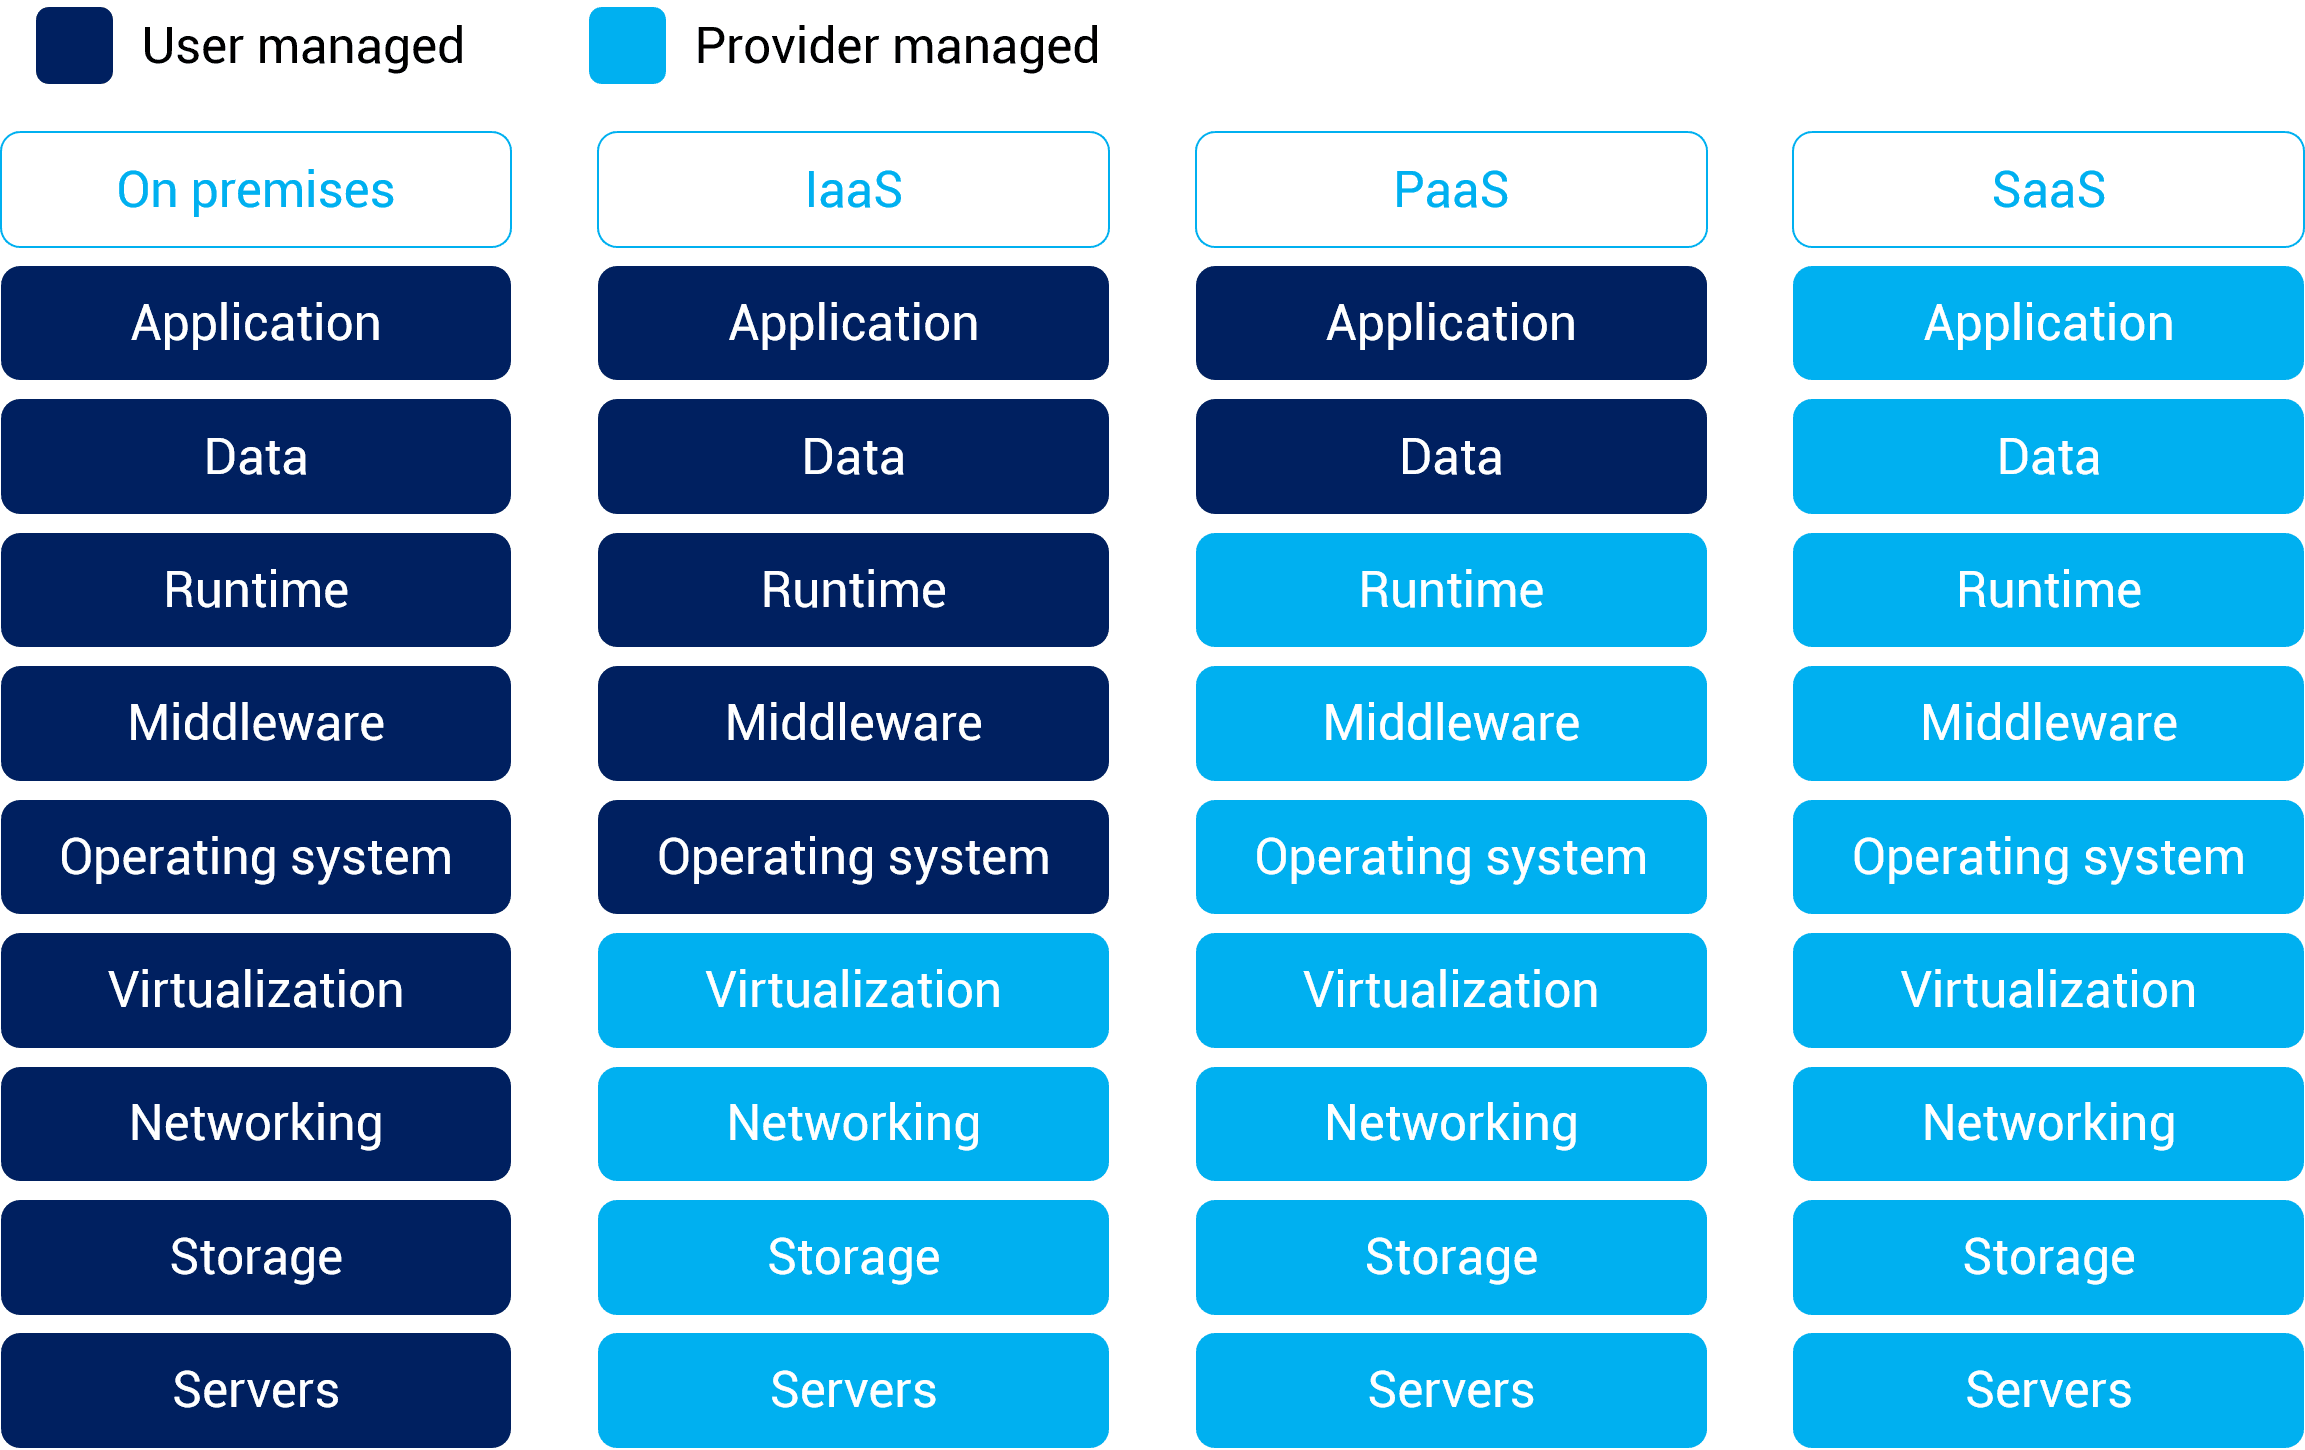
\includegraphics[width=0.5\textwidth]{bilder/iaas.png}
%\captionsetup[table]{justification=centering, labelfont=bf}
%\caption[On premises - IaaS - PaaS - SaaS]{On premises - IaaS - PaaS - SaaS\\Source: Alibaba Cloud \cite{alibaba}}
%\label{fig:iaas}
%\end{center}
%\end{figure}
%
%\textbf{Deployment models} \cite{Mell:2011:SND:2206223}
%\begin{itemize}
%    \item \textbf{Private cloud:} The infrastructure is exclusive to an organization. It can be owned and managed by the organization itself, but also by a third party. The private cloud can exist on or off premise.
%    \item \textbf{Community cloud:} A community cloud is very similar to a private cloud with the difference that it is provided for a specific community with common interests. It can be owned and managed by the community or a third party and can also be on or off premise.
%    \item \textbf{Public cloud:} The infrastructure is generally available to the public. It is typically owned and managed by the organization that runs it and is located on their premises.
%    \item \textbf{Hybrid cloud:} A hybrid cloud is a mixture of the above three types. Each type remains a separate unit, but is interconnected with the other units. In practice, this is often seen with companies who switch to a public cloud. They use a combination of private and public cloud and can therefore migrate application by application to the public cloud until all runs in the public cloud.
%\end{itemize}
%The German Federal Office for Information Security also shares this definition of cloud computing from the \gls{NIST} and has adopted it in principle more or less literally \cite{BSICC}.\\
%This thesis will be only treating public clouds and a slightly different service model called Function as a Service (\gls{FaaS}). It will be explained in the next section \ref{sec:serverless}.

%\textbf{Serverless Computing.}
%As defined by \gls{IBM} in \cite{serverlessibm}, "serverless is an approach to computing that offloads responsibility for common infrastructure management tasks (\emph{e.g.}, scaling, scheduling, patching, provisioning, etc.) to cloud providers and tools, allowing engineers to focus their time and effort on the business logic specific to their applications or process".
%Serverless requires less expertise than other self-managed approaches.
%Infact, users don't manage directly the operating infrastructure, delegating the (automatic) scaling directly to the cloud provider.
%This approach allows the providers to charge only for the given service offered~\cite{serverlessaws, serverlessazure}.

%Using serverless technologies requires much less expertise than non serverless self managed implementations. 
%Although those technologies might come with certain limitations or performance bottlenecks that won't fit to the user's needs.\\
%The most important key features of serverless computing are the following: 
%No server or infrastructure management of the user is required, the workload is scaled dynamically and automatically and it is usually paid per usage, e.g. only charged for the occupied storage in a service \cite{serverlessaws, serverlessazure}.\\
%There exists three main serverless offerings: \emph{(1)} FaaS (Function as a Service, \emph{e.g.}, \gls{AWS} Lambda), \emph{(2)} DBaaS (Database as a Service, \emph{e.g.} Microsoft Azure Database for PostgreSQL) and \emph{(3)} STaaS (Storage as a service, \emph{e.g.}, Google Cloud Storage \cite{serverlessgoogle}). 

%This thesis will treat the domain of FaaS.
%\subsection{FaaS (Function as a Service)}




%\subsection{Benchmarking}
%Benchmarking is a method to analyze and test the performance of a system, to discover its benefits and weaknesses and to compare it directly to other systems. 
%In this thesis, the systems will be serverless platforms and they will be tested with different applications to see how fast they run, how well they scale and how much they cost. 
%In order to get meaningful results, these tests should be executed as similar as possible on each system and repeated enough times to avoid coincidental data. In the following chapters the systems, the tests, the benchmark process and the results will be carefully discussed and explained in detail.

